\documentclass[12pt]{article}
\usepackage[T2A]{fontenc}
\usepackage[utf8]{inputenc}
\usepackage[russian, english]{babel}
\usepackage{amsmath}
\usepackage{amssymb}
\usepackage{amsthm}
\usepackage{amsfonts}
\usepackage[usenames]{color}
\usepackage{tikz}
\usepackage{comment}
\usepackage{hyperref}
\usepackage{blindtext}
\usepackage{centernot}
\usepackage{geometry}
\usepackage{subfig}
 \geometry{
 a4paper,
 total={170mm,257mm},
 left=20mm,
 top=20mm,
 }


\title{Тропические линейная алгебра}
\author{Никита Шапошник, Б05-025\\ научный руководитель: А. Э. Гутерман}

\newtheorem{theorem}{Теорема}[section]
\newtheorem{definition}[theorem]{Определение}
\newtheorem{proposition}[theorem]{Утверждение}
\newtheorem{remark}[theorem]{Замечание}
\newtheorem{lemma}[theorem]{Лемма}
\newtheorem{corollary}[theorem]{Следствие}
\newtheorem{algorithm}[theorem]{Алгоритм}

\date{}

\begin{document}
\maketitle

\section{Введение}
\begin{definition}
Тропическая алгебра (\cite{glanceOnTropicalLA},
        \cite{tropicalMath}) --- это множество $\mathbb{R}_{\max} = \mathbb{R} \cup \{ -\infty\}$ с операциями сложения $\oplus$ и умножения $\odot$: \begin{align*}
            a \oplus b &= \max(a, b)\\
            a \odot b &= a + b
        \end{align*}      
        или множество $\mathbb{R}_{min} = \mathbb{R} \; \cup \; \{ \infty\}$ с другой операцией сложения и идентичным умножением: \begin{align*}
            a \oplus b &= min(a, b)\\
            a \odot b &= a + b.
        \end{align*}
\end{definition}

В обоих случаях $0$ является нейтральным элементом по умножению, а бесконечные элементы --- нейтральными элементами по сложению.

В дальнейшем мы в основном будем работать с $\mathbb{R}_{\max}$.

Тропическая алгебра является полукольцом.

Множество матриц размера $n \times m$ над $\mathbb{R}_{\max}$ будем обозначать через $\mathbb{R}_{\max}^{n \times m}$. Для тропической матрицы $A$ будем писать $A > -\infty$, если в ней нет элементов, равных $-\infty$. 

Рассмотрим тропическую матрицу $A \in \mathbb{R}_{\max}^{n \times n}$. По ней можно построить ориентированный взвешенный граф $\mathcal{G}(A) = (V, E)$, где $V = \{ 1, 2, \dots, n\}$, а $E \subseteq V \times V$, где $(i, j) \in E$ тогда и только тогда, когда $a_{ij} \ne -\infty$. Веса рёбер определяются функцией $w : E \rightarrow \mathbb{R}$, $(i, j) \mapsto a_{ij}$. Говорят, что $A$ является матрицей смежности графа $\mathcal{G}(A)$.

Наоборот, по взвешенному ориентированному графу аналогично можно построить матрицу смежности. Для этого нужно пронумеровать вершины и поставить в соответствующие ячейки матрицы веса рёбер.

Кодирование графа тропической матрицей очень удобно. Например, по определению умножения матриц, легко доказать следующее утверждение. Зафиксируем квадратную тропическую матрицу $A$.

\begin{proposition}
\label{entriesInPower}
В ячейке матрицы $A^t$ с индексами $u, v$ лежит минимальный вес пути в графе $\mathcal{G}(A)$ от $u$ до $v$ длины ровно $t$.
\end{proposition}

Рассмотрим квадратную тропическую матрицу $A$.

\begin{definition}
Если существует целое неотрицательное $n$ такое, что $A^n > -\infty$, то матрица $A$ называется примитивной. В этом случае минимальное такое $n$ называется экспонентой матрицы $A$ и обозначается через $exp(A)$.
\end{definition}

\begin{definition}
Ориентированный граф $\mathcal{G}$ называется примитивным, если существует целое неотрицательное $n$ такое, что для любых двух вершин $u, v$ графа $\mathcal{G}$ существует путь от $u$ до $v$ длины ровно $n$. В этом случае минимальное такое $n$ называется экспонентой графа $\mathcal{G}$ и обозначается через $exp(\mathcal{G})$.
\end{definition}

Заметим, что, по утверждению \ref{entriesInPower}, примитивность матрицы $A$ эквивалентна примитивности графа $\mathcal{G}(A)$. Более того, $exp(A) = exp(\mathcal{G}(A))$.

Обозначим для произвольного графа $\mathcal{G}$ множество его вершин через $V(\mathcal{G})$, а множество его рёбер --- через $E(\mathcal{G})$.

\begin{definition}
Индекс цикличности (см. \cite{cyclicity}) (или просто цикличность) ориентированного графа $\mathcal{G}$ обозначается через $\sigma_\mathcal{G}$ и определяется следующим образом:
\begin{enumerate}
    \item Если $\mathcal{G}$ сильно связен, и $|V(\mathcal{G})| \ge 2$, то цикличность равна наибольшему общему делителю всех длин ориентированных циклов в $\mathcal{G}$.
    \item Если в $\mathcal{G}$ есть только одна вершина (с петлей или без), то $\sigma_\mathcal{G} = 1$.
    \item Если $\mathcal{G}$ не сильно связен, то его цикличность равна наименьшему общему кратному цикличностей всех максимальных его сильно связных подграфов.
\end{enumerate}
\end{definition}

С помощью индекса цикличности можно написать критерий примитивности ориентированного графа:

\begin{theorem}[\cite{Brualdi}]
Ориентированный граф $\mathcal{G}$ примитивен тогда и только тогда, когда $\mathcal{G}$ сильно связен и его индекс цикличности равен $1$.
\end{theorem}

Заметим, что в сильно связном графе $\mathcal{G}$ с цикличностью $\sigma$ любые два пути, соединяющие две фиксированные вершины, имеют одинаковые длины по модулю $\sigma$. Из этого следует, что на множестве $V(\mathcal{G})$ можно ввести отношение эквивалентности: две вершины лежат в одном классе эквивалентности тогда и только тогда, когда длина пути от одной к другой кратна $\sigma$. Эти классы эквивалентности называются циклическими классами.

Пусть $\mathcal{G} = (V, E)$ --- взвешенный ориентированный граф с матрицей смежности $A = (a_{ij}) \in \mathbb{R}_{\max}^{n \times n}$. Пусть $C$ --- это ориентированный цикл в $\mathcal{G}$ с весами ребер $a_{i_1}, a_{i_2}, \dots, a_{i_l}$. Средний вес ребра в $C$ --- это тропическое среднее геометрическое весов ребер в $C$:
\begin{equation*}
    w_a(C) = \sqrt[\odot l]{a_{i_1} \odot a_{i_2} \odot \dots \odot a_{i_l}}=
    \frac{1}{l}(a_{i_1} + a_{i_2} + \dots + a_{i_l})
\end{equation*}
\begin{definition}
Ориентированный цикл называется критическим, если у него максимальный средний вес. Критический подграф $\mathcal{G}^c$ графа $\mathcal{G}$ --- это объединение всех критических циклов в $\mathcal{G}$.
\end{definition}

Обозначим максимальный средний вес цикла в $\mathcal{G}(A)$ через $\lambda(A)$, т.е.
\begin{equation*}
    \begin{split}
        \lambda(A) = \bigoplus_{k = 1}^d \bigoplus_{i_1, \dots, i_k} (a_{{i_1}{i_2}}\odot \dots \odot a_{{i_{k - 1}}{i_k}})^{\odot{1/k}} =\\
        =\max_{k = 1}^d \max_{i_1, \dots, i_k} \frac{(a_{{i_1}{i_2}} + \dots + a_{{i_{k - 1}}{i_k}})}{k}
    \end{split}
\end{equation*}

Назовем тропическую матрицу $A$ (или соответствующий ей граф) неразложимой, если граф $\mathcal{G}(A)$ сильно связен, иначе --- разложимой.

Назовем тропическую матрицу $A$ (или соответствующий ей граф) полностью разложимой, если в графе $\mathcal{G}(A)$ нет ребер между различными компонентами сильной связности.

Рассмотрим тропическую матрицу $A \in \mathbb{R}_{\max}^{n \times n}$. Тогда звездой Клини матрицы $A$ называется следующая матрица:

\begin{equation*}
    A^* = \bigoplus_{i = 0}^{\infty} A^i =  \bigoplus_{i = 0}^{n - 1} A^i
\end{equation*}

В матрице $A^*$ в ячейке под номером $i$ и $j$ лежит длина оптимального пути от вершины $i$ к вершине $j$ в графе $\mathcal{G}(A)$ без ограничения на длину пути. Условие $\lambda(A) \le 0$ необходимо, так как иначе этот ряд расходится: можно идти по циклу с положительным средним весом и улучшать ответ. Так как дважды проходить через одну и ту же вершину не имеет смысла, можно ограничиться первыми $n$ матрицами.

Обхватом графа $\mathcal{G}$ называется наименьшая длина цикла в $\mathcal{G}$ и обозначается как $g(\mathcal{G})$. Через $\hat{g}(\mathcal{G})$ обозначается максимальный обхват среди всех компонент сильной связности графа $\mathcal{G}$.

Окружностью графа $\mathcal{G}$ называется наибольшая длина цикла в $\mathcal{G}$ и обозначается как $cr(\mathcal{G})$ (от английского circumference).

Максимальную длину простого пути в графе $\mathcal{G}$ будем обозначать через $cd(\mathcal{G})$ (от английского cab-driver's diameter).

\section{CSR-разложение}
\label{subsection:CSR}
Рассмотрим неразложимую $A \in \mathbb{R}_{\max}^{n \times n}$. Введем обозначения: $\sigma = \sigma(\mathcal{G}^c(A))$ -- индекс цикличности критического подграфа, $M = ((\lambda(A)^-\odot A^\sigma)^*$. Здесь и далее для $a \in \mathbb{R}_{\max}$, $a \ne -\infty$ через $a^-$ будем обозначать обратное по умножению к $a$, т.е. $a^- = -a$.

Определим матрицы $C, S, R \in \mathbb{R}_{\max}^{n \times n}$ следующим образом:
\begin{align*}
    c_{ij} &= \begin{cases}
        m_{ij}\text{, если } j \in V(\mathcal{G}^c(A)) \\
        -\infty \text{, иначе,}
    \end{cases}
    &
    r_{ij} = \begin{cases}
        m_{ij}\text{, если } i \in V(\mathcal{G}^c(A)) \\
        -\infty \text{, иначе,}
    \end{cases}
    \\
    s_{ij} &= \begin{cases}
        \lambda(A)^- \odot a_{ij}\text{, если } (i, j) \in E(\mathcal{G}^c(A)) \\
        -\infty \text{, иначе.}
    \end{cases}
\end{align*}

Если матрицы $C, S, R$ определены по матрице $A$, будем писать $CS^tR[A]$ для произвольного $t$.
\begin{theorem}[\cite{bounds}, \cite{15WeakCSRExpantion}]
\label{theorem:CSRdecompositionTheorem}
Пусть $A \in \mathbb{R}_{\max}^{n \times n}$ неразложима. Тогда существует неотрицательное целое $T(A)$ такое, что для любого $t \ge T(A)$:
\begin{equation}
\label{equation:TDefinition}
    A^t = \lambda(A)^{\odot t} \odot CS^tR[A].
\end{equation}
\end{theorem}

Заметим, что если $\lambda(A) = 0$, то (\ref{equation:TDefinition}) записывается в виде:
\begin{equation*}
    A^t = CS^tR[A].
\end{equation*}

\begin{proposition} [\cite{21CSRExpansionsOfMatrixPowersInMaxAlgebra}] \label{periodicity}
Для любого $t \ge 0$ верно, что 
$CS^{t+\sigma}R[A] = CS^tR[A]$, где $\sigma$ --- это цикличность $\mathcal{G}^c(A)$. Иначе говоря, последовательность матриц $\{ CS^tR[A]\}_{t\ge0}$ периодична с периодом $\sigma$.
\end{proposition}

Значит, в силу равенства $A^t = CS^tR$ при $t \ge T(A)$, последовательность матриц $A^t$ при $t \ge T(A)$ является периодической с периодом $\sigma$.

Через $\mathcal{W}^{t, l}(i \xrightarrow{\mathcal{G}'} j)$ обозначим множество путей от вершины $i$ к вершине $j$, имеющих длину $t$ по модулю $l$, и проходящих хотя бы через одну вершину графа $\mathcal{G}'$. Для множества $\mathcal{W}$ через $p(\mathcal{W})$ обозначим максимальный вес пути из множества $\mathcal{W}$.

\begin{proposition}[\cite{15WeakCSRExpantion}] \label{entriesInCSR}
Если $\lambda(A) = 0$, то верно следующее равенство:
\begin{equation}
    (CS^tR[A])_{ij} = p(\mathcal{W}^{t, \sigma}(i \xrightarrow{\mathcal{G}^c(A)} j)),
\end{equation}
где $\sigma$ обозначает цикличность $\mathcal{G}^c(A)$.
\end{proposition}

Введём ещё одну функцию --- $T_{1, N}(A)$. Для этого определим матрицу $B \in \mathbb{R}_{\max}^{n \times n}$:
\begin{equation*}
    b_{ij} = 
    \begin{cases}
        -\infty \text{, если $i \in V(\mathcal{G}^c)$ или $j\in V(\mathcal{G}^c)$}, \\
        a_{ij}, \text{ иначе.}
    \end{cases}
\end{equation*}

\begin{theorem}[\cite{bounds}, \cite{15WeakCSRExpantion}]
\label{theorem:weakCSRexpantionTheorem}
Пусть $A \in \mathbb{R}_{\max}^{n \times n}$ неразложима. Тогда существует неотрицательное целое $T_1(A, B)$  такое, что для любого $t \ge T_1(A, B)$:
\begin{equation}
\label{equation:T1definition}
    A^t = (\lambda(A)^{\odot t} \odot CS^tR[A]) \oplus B^t.
\end{equation}
\end{theorem}

Заметим, что если $\lambda(A) = 0$, то (\ref{equation:T1definition}) записывается в виде $A^t = CS^tR[A] \oplus B^t$, и если $B = -\infty$, то $T(A) = T_1(A, B)$.

\begin{remark}[Инвариантность относительно умножения на скаляр]
\label{invarianceOfT}
Если $A' = A \odot \mu$, где $\mu \ne -\infty$, то

\begin{itemize}
	\item $\lambda(A') = \lambda(A) \odot \mu$, $B_N[A'] = B_N[A]$
	\item $CSR[A'] = CSR[A]$
\end{itemize}

Значит, $T(A)$ и $T_1(A, B)$ инвариантны относительно умножения матрицы на конечный скаляр, что позволяет нам без разграничения общности говорить, что $\lambda(A) = 0$.
\end{remark}

Есть множество способов определить матрицу $B$, здесь мы рассматриваем лишь частный случай. Обозначим $T(A, B)$ для описанной матрицы $B$ через $T_{1, N}(A)$.

Существуют несколько оценок для $T_{1, N}(A)$. В дальнейшем мы будем рассматривать только графы, в которых все рёбра имеют нулевой вес, поэтому $B = 0$. Следовательно, $T(A) = T_{1, N}(A)$, и оценки для $T_{1, N}(A)$ верны и для $T(A)$.

\begin{theorem}[Верхние оценки $T_{1, N}(A)$, \cite{15WeakCSRExpantion}]
Для любой $A \in \mathbb{R}_{\max}^{n \times n}$ имеем:
\begin{enumerate} 
    \item $T_{1, N}(A) \le Wi(n)$;
    \item $T_{1, N}(A) \le \hat{g}(n - 2) + n$;
    \item $T_{1, N}(A) \le (\hat{g} - 1)(cr - 1) + (\hat{g} + 1) cd$,
\end{enumerate}
где $\hat{g} = \hat{g}(\mathcal{G}^c(A))$, $cr = cr(\mathcal{G}(A))$, а $cd = cd(\mathcal{G}(A))$.
\end{theorem}

\begin{corollary}[Верхние оценки $T(A)$]
\label{upperBounds}
Для любой неразложимой $A \in \mathbb{R}_{\max}^{n \times n}$ имеем:
\begin{enumerate} 
    \item $T(A) \le Wi(n)$;
    \item $T(A) \le \hat{g}(n - 2) + n$;
    \item $T(A) \le (\hat{g} - 1)(cr - 1) + (\hat{g} + 1) cd$,
\end{enumerate}
где $\hat{g} = \hat{g}(\mathcal{G}^c(A))$, $cr = cr(\mathcal{G}(A))$, а $cd = cd(\mathcal{G}(A))$.
\end{corollary}



\section{Примеры}
\subsection{Полный граф}
Рассмотрим матрицу $A \in \mathbb{R}_{\max}^{n \times n}$, где $a_{ij} = 0$ для любых индексов $i, j$. Граф $\mathcal{G}(A)$ является полным, веса всех ребер в нём равны $0$. Значит, критический подграф $\mathcal{G}^c$ совпадает со всем графом $\mathcal{G}$.

Найдем матрицы $C, S, R$. Индекс цикличности полного графа $\sigma = 1 $ (т.к. в нём есть циклы длины $1$), следовательно $C = R = M = A^*$, $S = A$.

Так как для любого положительного $t$ верно, что $A^t = A$, то $A^* = A$ и равенство $A^*A^tA^* = A^t$ выполняется для любого положительного $t$.

Следовательно, $T = 1$.

\subsection{Односторонний цикл}
\begin{figure}[h]
% \caption{Односторонний цикл.}
  \centering
    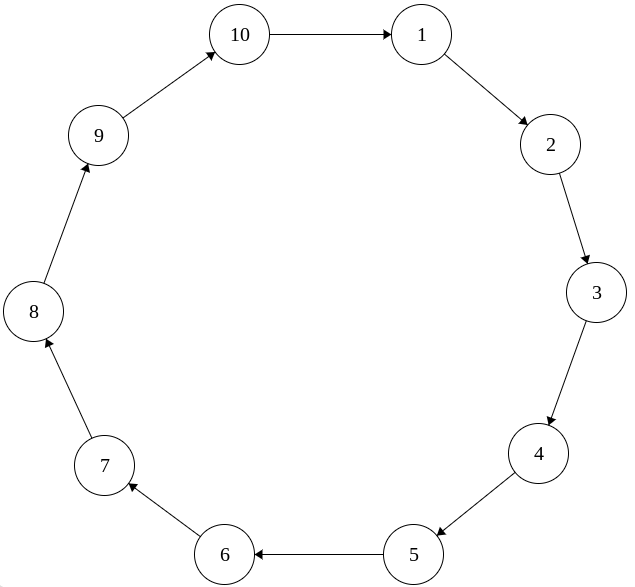
\includegraphics[width=0.6\textwidth]{ForwardCycle}
\end{figure}

Рассмотрим матрицу смежности $A \in \mathbb{R}_{\max}^{n \times n}$ одностороннего цикла на $n$ вершинах.

В силу инвариантности границ относительно домножения на скаляр из $\mathbb{R}$ (замечание \ref{invarianceOfT}), можно рассматривать только тот случай, в котором $\lambda(A) = 0$.
Тогда $\mathcal{G}^c(A) = \mathcal{G}(A)$, $\sigma = n$.
\begin{equation*}
M = (A^n)^* = E^* = E = \begin{pmatrix}
0 & -\infty & ... & -\infty \\
-\infty & 0 & ... & -\infty \\
... & ... & ... & ... \\
-\infty & -\infty & ... & 0
\end{pmatrix} = diag(0, 0, \dots, 0)
\end{equation*}
Значит, $C = R = E$, $S = A$, и для любого неотрицательного $t$ верно $CS^tR[A] = A^t$. Следовательно, $T = 0$.

\subsection{Двусторонний цикл}
\begin{figure}[h]
% \caption{Односторонний цикл.}
  \centering
    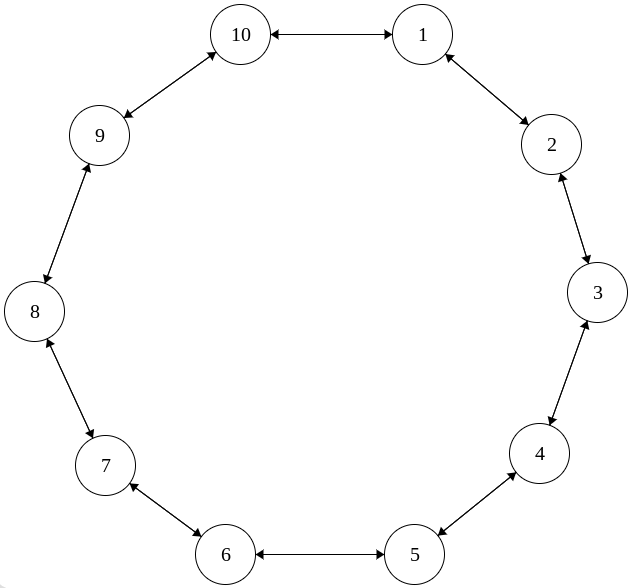
\includegraphics[width=0.6\textwidth]{BidirectionalCycle}
\end{figure}

Рассмотрим матрицу смежности $A \in \mathbb{R}_{\max}^{n \times n}$ двустороннего цикла на $n$ вершинах, все рёбра в котором имеют нулевой вес, тогда $\lambda(A) = 0$ и $\mathcal{G}^c(A) = \mathcal{G}(A)$. Пронумеруем вершины так, чтобы первый цикл состоял из вершин $1, 2, \dots n$(в порядке обхода), а второй --- из $n, n - 1, \dots, 1$ (в порядке обхода). Чтобы избежать кратных рёбер, будем работать с $n \ge 3$.

Необходимо рассмотреть два случая: когда $n$ нечётно и когда $n$ чётно.

\textbf{n нечетно.} В этом случае цикличность критического графа $\sigma = 1$, т.е. граф примитивен. Значит, $T(A) = exp(A)$.

\begin{proposition}
Экспонента данного графа равна $n - 1$.
\end{proposition}
\begin{proof}[\textbf{Доказательство.}]
Заметим, что в $A^{n - 2}$ на главной диагонали стоят $-\infty$: $n - 2$ нечётно, поэтому, чтобы вернуться в исходную вершину за $n - 2$ шага, надо сменить чётность --- пройти весь круг, так как остальные циклы имеют чётную длину. Но цикл имеет длину $n$, поэтому его пройти не получится. Значит, $exp(\mathcal{G}) \ge n - 1$.

Покажем, что $A^{n - 1} > -\infty$.

Зафиксируем произвольную вершину $v$ графа. Назовем вершину \textit{четной}, если до нее можно дойти из $v$ за чётное число шагов. Заметим, что тогда все вершины графа четные, так как $n$ нечетно и идти можно как по, так и против часовой стрелки. Наибольшая длина такого пути равна $n - 1$. Значит, $A^{n - 1} > -\infty$.
\end{proof}

\textbf{n четно.} В этом случае $\sigma = 2$ и граф не примитивен. $C = R = M = (A^2)^*$, $S = A$.

Так как последовательность матриц $CS^tR$ периодична с периодом $\sigma = 2$ (см. \cite{15WeakCSRExpantion}), то при $t \ge T(A)$ \begin{equation*}
A^t = CS^tR = \begin{cases}
(A^2)^* \text{, если } t \text{ четно.}\\
A \odot (A^2)^*\text{, если } t \text{ нечетно.}\\
\end{cases}
\end{equation*}
В матрице $(A^2)^*$ небесконечные элементы стоят в клетках $(i, j)$, если вершины $i$ и $j$ находятся на четном расстоянии друг от друга. Наибольшее расстояние между вершинами с одинаковой четностью равно $\frac{n}{2}$. Значит, условие при четном $t$ выполняется при $t \ge \frac{n}{2}$, а при прочих $t$ не выполняется.

В матрице $A\odot(A^2)^*$ небесконечные элементы стоят в клетках $(i, j)$, если вершины $i$ и $j$ находятся на нечетном расстоянии друг от друга. Наибольшее расстояние между вершинами с разной четностью равно $\frac{n}{2} - 1$. Значит, условие при четном $t$ выполняется при $t \ge \frac{n}{2} - 1$, а при прочих $t$ --- не выполняется.

Следовательно, $T(A) = \frac{n}{2}$.

\subsection{Примитивные графы с нулевыми рёбрами}
Функция $T$ является обобщением экспоненты на непримитивные графы.

Рассмотрим примитивный граф с матрицей смежности $A$, в котором вес каждого ребра равен $0$. Тогда критический подграф совпадает со всем графом, и индекс цикличности примитивного графа $\sigma = 1$.

По утверждению \ref{periodicity} последовательность матриц $CS^tR[A]$ периодична с периодом $\sigma = 1$, то есть в этой последовательности все члены равны. Из утверждения \ref{entriesInCSR} и примитивности $A$ следует, что матрица $CS^tR[A]$ целиком состоит из $0$ при любом $t$.

Заметим, что в любой степени матрицы $A$ её элементы будут принимать только два значения: $-\infty$ и $0$. Из определения $T(A)$ следует, что $A^t = CS^tR[A]$ тогда и только тогда, когда $t \ge T(A)$. Значит, матрица $A^t$ не содержит $-\infty$ тогда и только тогда, когда $t \ge T(A)$. Значит, $T(A) = exp(A)$, если $A$ примитивна.

Это приводит нас к более общему утверждению.

\begin{proposition} \label{onePathProposition}
Рассмотрим примитивную матрицу $A$, у которой $\mathcal{G}(A)$ совпадает со своим критическим подграфом, $\lambda(A) = 0$. Если для двух произвольных фиксированных вершин $u$ и $v$ верно, что все пути из $u$ в $v$ имеют одинаковый вес, то $T(A) = exp(A)$.
\end{proposition}
\begin{proof}[\textbf{Доказательство.}]
В силу условия на одинаковый вес между любыми двумя вершинами матрицы вида $CS^tR[A]$ принимают только одно значение (по утверждению \ref{entriesInCSR}), а значение конкретной ячейки матрицы $A^t$ либо равно $-\infty$, либо совпадает с соответстующей ячейкой $CS^tR[A]$. Значит, условие $A^t = CS^tR[A]$ равносильно условию $A^t > -\infty$. Следовательно, $T(A) = exp(A)$.
\end{proof}

Заметим, что обратное утверждение неверно. Рассмотрим следующие графы:

\begin{figure}[h]%
    \centering
    \subfloat[\centering]{{\includegraphics[width=6cm]{9.7_Counter1} }}%
    \qquad
    \subfloat[\centering]{{\includegraphics[width=6cm]{9.7_Counter2} }}%
    \label{fig:example}%
\end{figure}

В обоих графах экспонента совпадает с $T$ (в обоих графах экспонента равна $2$), но в графе (a) максимальный средний вес цикла равен $-1$, а в графе (b) критический подграф не совпадает со всем графом.

Рассмотрим неразложимую матрицу $A$ такую, что в $\mathcal{G}(A)$ все рёбра имеют нулевой вес. Пусть его индекс цикличности равен $\sigma$.

\section{Граница T для ромашек}
\begin{definition} Назовем ромашкой граф, состоящий из нескольких пересекающихся по одной вершине циклов.
\end{definition}

Здесь и далее будем рассматривать графы-ромашки, состоящие из циклов длины, кратной $\sigma$, все рёбра в которых имеют вес $0$.

\begin{definition}
Ромашку, состоящую из циклов длины $a_1\sigma, a_2\sigma, \dots, a_n\sigma$, где числа $a_1, \dots, a_n$ взаимно просты в совокупности, $a_1\le a_2 \le \dots \le a_n$ назовем $(a_1, \dots, a_n; \sigma)$-ромашкой.

Границу $T$, определенную для такой ромашки, будем обозначать через $T(a_1, \dots, a_n; \sigma)$.
\end{definition}

Заметим, что индекс цикличности такой ромашки равен $\sigma$ и всего в ней $N = \sum\limits_{\substack{i=1}}^n a_i\sigma - n + 1$ вершин. Пусть вершина, в которой пересекаются все циклы, имеет номер $1$. Пронумеруем вершины в порядке следующего обхода: начнем в вершине $1$, далее пройдём по первому циклу, затем --- по второму, и так далее до цикла с номером $n$ (не изменяя номер у вершины $1$).

Во всех примерах матрицу смежности рассматриваемого графа будем обозначать через $A \in \mathbb{R}_{\max}^{n \times n}$, а через $C, S, R$ будем обозначать матрицы $C, S, R$, построенные по матрице $A$.

\begin{theorem}
\label{everyKFormula}
$T(a_1, \dots, a_n; \sigma) = (T(a_1, \dots, a_n; 1) + 1)\sigma - 1$.
\end{theorem}
\begin{proof}[\textbf{Доказательство}] 
Обозначим граф, соответствующий $(a_1, \dots, a_n; 1)$-ромашке через $\mathcal{G}$, а граф, соответствующий $(a_1, \dots, a_n; \sigma)$-ромашке --- через $\mathcal{G}_\sigma$. Граф $\mathcal{G}_\sigma$ получается из графа $\mathcal{G}$ разделением каждого ребра на $\sigma$ более мелких рёбер. Вершины $\mathcal{G}_\sigma$, лежащие в одном циклическом классе с вершиной $1$, будем называть начальными. Для краткости будем обозначать $T(a_1, \dots, a_n; 1)$ через $T^1$, а $T(a_1, \dots, a_n; \sigma)$ --- через $T^{\sigma}$.

Покажем, что $T^{\sigma} > (T^1 + 1)\sigma - 2$. В $\mathcal{G}$ есть $2$ вершины, между которыми нет пути длины $T^1 - 1$. Значит, в $\mathcal{G}_\sigma$ между соответствующими начальными вершинами нет пути длины $(T^1 - 1)\sigma$. Обозначим эти вершины через $u$ и $v$. Но тогда между вершинами $\hat{u}$ и $\hat{v}$ не будет пути длины $(T^1 - 1)\sigma + 2(\sigma - 1) = (T^1 + 1)\sigma - 2$, где $\hat{u}$ получается, если отойти от $u$ на $\sigma - 1$  шаг вперёд, а $\hat{v}$ --- от вершины $v$ на $\sigma - 1$ шаг назад (обе новые вершины существуют, так как любая вершина в $\mathcal{G}$ лежит в цикле). Значит, $T^{\sigma} \ge (T^1 + 1)\sigma - 1$.

Покажем, что $T^{\sigma} \le (T^1 + 1)\sigma - 1$. Для этого нужно доказать, что между любыми двумя вершинами $u$ и $v$ графа $\mathcal{G}_\sigma$ есть путь длины $(T^1 + 1)\sigma - 1$ от $u$ до $v$. Путь длины $(T^1 + 1)\sigma - 1$ от $u$ до $v$ состоит из трех частей: путь от $u$ до ближайшей начальной вершины, путь между начальными вершинами, и путь от ближайшей начальной вершины до $v$. Суммарная длина первой и третьей частей не превосходит $2\sigma - 2$, значит, длина второй части не меньше $(T^1 - 1)\sigma + 1$. Но длина пути между двумя начальными вершинами должна быть кратна $\sigma$, поэтому длина второй части не меньше $T^1\cdot \sigma$. Но, по определению $T^1$, между любыми начальными вершинами есть путь длины $T^1\cdot \sigma$. Значит, $T^{\sigma} \ge (T^1 + 1)\sigma - 1$, и утверждение доказано.
\end{proof}
Таким образом, при расчёте границы $T$ для произвольной ромашки достаточно посчитать искомую границу при $\sigma = 1$, а затем получить ответ по формуле из утверждения \ref{everyKFormula}. 

\begin{remark}
\label{rmrk:expAndT}
При $\sigma = 1$ $(a_1, \dots, a_n; 1)$-ромашка примитивна, все рёбра в ней имеют нулевой вес. Значит, граница $T$ ромашки совпадает её экспонентой.
\end{remark}

Введём вспомогательную функцию $P$:
\begin{definition}
Для взаимно простых в совокупности натуральных чисел $a_1 \le \dots \le a_n$ обозначим через $P(a_1, \dots, a_n)$ минимальное целое неотрицательное число, удовлетворяющее следующему свойству: любое $p \ge P(a_1, \dots, a_n)$ выражается в виде линейной комбинации чисел $a_1, \dots, a_n$ с целыми неотрицательными коэффициентами $\lambda_1, \dots, \lambda_n$, то есть
\begin{equation}
\label{LK}
p = a_1 \lambda_1 + \dots a_n \lambda_n.
\end{equation}
Число, выражающееся в виде линейной комбинации чисел $a_1, \dots, a_n$ с целыми \\ неотрицательными коэффициентами, назовём выразимым.
\end{definition}

Здесь и далее под линейной комбинацией будем понимать линейную комбинацию с целыми неотрицательными коэффициентами.

\begin{theorem}
\label{thTP}
$T(a_1, \dots, a_n; 1) = P(a_1, \dots, a_n) + 2a_n - 2$.
\end{theorem}
\begin{proof}[\textbf{Доказательство.}]
По определению границы $T$ для любых двух вершин между ними существует путь длины $t$ для любого $t \ge T(a_1, \dots, a_n; 1)$, и сущесвуют две вершины, между которыми нет пути длины $T(a_1, \dots, a_n; 1) - 1$.

Рассмотрим две произвольные вершины $u$ и $v$. Любой путь длины хотя бы $a_n - 1$ проходит через вершину $1$. Поэтому путь длины $t$ от $u$ до $v$ состоит из трёх частей: пути от $u$ до $1$ (обозначим длину этой части через $\hat{u}$), $\lambda_i$ циклов длины $a_i$ для $i = 1\dots n$, и пути от $1$ до $v$ (обозначим длину этой части через $\hat{v})$. Тогда имеет место равенство:
\begin{equation*}
    t = \hat{u} + a_1 \lambda_1 + \dots + a_n \lambda_n + \hat{v} \quad \Longleftrightarrow \quad t - \hat{u} - \hat{v} = a_1 \lambda_1 + \dots + a_n \lambda_n.
\end{equation*}
Сумма $\hat{u} + \hat{v}$ принимает любые значения от $0$ до $2a_n - 2$ (так как $0 \le \hat{u}, \hat{v} \le a_n - 1$). Следовательно, любое число $p$ такое, что $t - 2a_n + 2 \le p \le t$, должно быть выразимо.

При $t < P(a_1, \dots, a_n) + 2a_n - 2$ минимальное значение $p$ не превосходит $P(a_1, \dots, a_n) - 1$, и, по определению $P(a_1, \dots, a_n)$, при наименьшем значении $p$ уравнение \ref{eqTP} решений не имеет --- противоречие с наличием пути между $u$ и $v$.

Напротив, при $t \ge P(a_1, \dots, a_n) + 2a_n - 2$ наименьшее значение $p$ не меньше $P(a_1, \dots, a_n)$, и, в силу определения $P(a_1, \dots, a_n)$, коэффициенты $\lambda_i$ найдутся для любого возможного значения $p$.

Значит, $T(a_1, \dots, a_n; 1) = P(a_1, \dots, a_n) + 2a_n - 2$.
\end{proof}

\begin{corollary}[Корректность функции $P$]
Функция $P$ определена корректно: её значение существует для любых подходящих аргументов.
\end{corollary}
\begin{proof}[\textbf{Доказательство.}]
Рассмотрим $(a_1, \dots, a_n; 1)$-ромашку. По замечанию \ref{rmrk:expAndT} этот граф примитивен и, следовательно, имеет экспоненту, которая, в свою очередь, совпадает с границей $T$ для данной ромашки. По формуле из теоремы \ref{thTP} имеем $P(a_1, \dots, a_n) = T(a_1, \dots, a_n; 1) - 2a_n + 2$.
\end{proof}

\begin{proposition}[Свойства функции $P$]{\ }
\label{propertiesOfP}
\begin{enumerate}
    \item Если $a_1 = 1$, то $P(1, \dots, a_n) = 0$.
    \item $P(a_1, \dots, a_n) \le P(a_{i_1} , a_{i_2}, \dots, a_{i_k})$, где $1 \le i_1 < i_2 < \dots < i_k \le n$ --- возрастающая последовательность индексов.
    \item $P(a_1, \dots, a_n) = P(b_1, \dots, b_m)$, где набор $b_1, \dots, b_m$ получается из набора $a_1, \dots, a_n$ удалением повторяющихся элементов.
    \item Если $a_j$ делится на $a_i$, то $P(a_1, \dots, a_n) = P(a_1, \dots, a_{j - 1}, a_{j + 1}, \dots, a_n)$.
    
    \item Если $a_j$ представляется в виде линейной комбинации меньших элементов, то \\
     $P(a_1, \dots, a_n) = P(a_1, \dots, a_{j - 1}, a_{j + 1}, \dots, a_n)$.
\end{enumerate}
\end{proposition}
\begin{proof}[\textbf{Доказательство.}]
1) Действительно, если $a_1 = 1$, то любое неотрицательное число $k$ выражается как $1 \cdot k$. Следовательно, $P = 0$.

2) Свойство следует из следующего факта: сумма $a_{i_1} \lambda_{i_1} + \dots + a_{i_k}\lambda_{i_k}$ является частным случаем суммы $a_1 \lambda_1 + \dots + a_n \lambda_n$.

3) При приведении подобных членов в сумме $a_1 \lambda_1 + \dots + a_n \lambda_n$ получается корректная сумма $b_1 \mu_1 + \dots b_m \mu_m$. С другой стороны, сумма $b_1 \mu_1 + \dots b_m \mu_m$ является корректной суммой вида $a_1 \lambda_1 + \dots + a_n \lambda_n$.

4) Очевидно, что любая сумма $a_1 \lambda_1 + \dots + a_{j - 1} \lambda_{j - 1} + a_{j + 1} \lambda_{j + 1} + \dots +a_n \lambda_n$ является суммой вида $a_1 \lambda_1 + \dots + a_n \lambda_n$, где $\lambda_j = 0$. С другой стороны, заменив $a_j$ на $a_i \cdot \frac{a_j}{a_i}$, можно избавиться от слагаемого $a_j \lambda_j$ в сумме $a_1 \lambda_1 + \dots + a_n \lambda_n$, что доказывает утверждение.

5) Доказетельство этого свойства аналогично предыдущему.
\end{proof}

\begin{proposition}
$P(a, b) = (a - 1)(b - 1)$.
\end{proposition}
\begin{proof}[\textbf{Доказательство}]
Покажем, что $p = ab - a - b \ne ma + nb$ для любых целых неотрицательных $m, n$.

Предположим противное. Тогда: \begin{equation*}
 ab - a - b = am + bn \quad \Longleftrightarrow \quad ab = (m + 1)a + (n + 1) b
\end{equation*}
В силу взаимной простоты $a$ и $b$ получим, что $n + 1 \ \vdots \ a$, и $m + 1 \ \vdots \ b$. Тогда, в силу того, что $m, n \ge 0$, имеем $2$ случая:\begin{align*}
     \begin{cases}
        n + 1 = a\\
        m + 1 = 0
    \end{cases}
    &
    \begin{cases}
        n + 1 = 0\\
        m + 1 = b.
    \end{cases}
\end{align*}
В обоих случаях получаем противоречие. Следовательно, $P(a, b) \ge (a - 1)(b - 1)$.

Теперь покажем, что $P(a, b) \le ab + b - a - 1$. Для любого $p \ge ab - b - a + 1$ решим уравнение: \begin{equation*}
am + bn = p
\end{equation*}
Так как $a$ и $b$ взаимно просты, числа из набора $0, b, 2b, \dots, (a - 1)b$ дают все $a$ остатков по модулю $a$. Значит, существует единственное $0 \le n \le a - 1$, что $bn \equiv p \pmod a$, причём $p - bn \ge 0$, так как $p - bn \ \vdots \ a$ и
\begin{equation*}
p - bn \ge ab - b - a + 1 - (a - 1)b = -a + 1 > -a \Longrightarrow p - bn \ge 0.
\end{equation*}
Значит, $m = \frac{p - bn}{a} \ge 0$.

Таким образом, нами были найдены целые $m \ge 0$, $n \ge 0$. Следовательно, $P(a, b) = (a - 1)(b - 1)$.
\end{proof}
\begin{corollary}
$T(a, b; \sigma) = (ab + b - a)\sigma - 1$.
\end{corollary}

\begin{proposition}
$P(2, a, b) = \begin{cases}
P(2, b) = b - 1, &\text{если $a$ чётно,} \\
P(2, a) = a - 1,&\text{иначе.}
\end{cases}$
\end{proposition}
\begin{proof}[\textbf{Доказательство}]
Первый случай следует из свойства 4 утверждения \ref{propertiesOfP}.

Разберём второй случай: $a$ нечётно. Неравенство $P(2, a, b) \le P(2, a)$ следует из свойства $2$ утверждения \ref{propertiesOfP}. Докажем обратное неравенство: необходимо показать, что с помощью слагаемых $2, a, b$ невозможно получить сумму $a - 2$. Действительно, из трёх слагаемых можно использовать только одно: $2$. Но $a - 2$ нечётно --- противоречие. Следовательно, $P(2, a, b) = P(2, a)$.
\end{proof}

\begin{corollary}
$T(2, a, b; \sigma) = \begin{cases}
T(2, b; \sigma) = (3b - 2)\sigma - 1, &\text{если $a$ нечётно,} \\
(2b + a - 2)\sigma - 1, &\text{иначе.}
\end{cases}$
\end{corollary}

Чтобы легче вычислять функцию $P$, определим вспомогательную функцию $M$, сопоствяляющую каждому целому числу от $0$ до $a_1 - 1$ целое неотрицательное число: $M[i]$ --- это минимальное выразимое число, сравнимое с $i$ по модулю $a_1$. Впоследствии, при описании алгоритма, вычисляющего $P$, удобно будет представлять $M$ в качестве массива, поэтому значение функции $M$ на элементе $i$ будем обозначать с помощью квадратных скобок --- через $M[i]$.

Заметим, что $M[0] = 0$ и что $M[i] \equiv i \pmod {a_1}$.

\begin{proposition}
\label{algorithm:lemma1}
$P(a_1, \dots, a_n) = \max\limits_{i = 0}^{a_0 - 1} M[i] - a_1 + 1$.
\end{proposition}
\begin{proof}[\textbf{Доказательство}]
Пусть $\max\limits_{i = 0}^{a_0 - 1} M[i] = M[k]$.

Выразимость $M[k] - a_1$ вела бы к противоречию с определением массива $M$, так как $M[k] - a_1 \equiv M[k] \pmod {a_1}$. Значит, $P(a_1, \dots, a_n) \ge \max\limits_{i = 0}^{a_0 - 1} M[i] - a_1 + 1$.

Заметим, что если произвольное $x$ выразимо, то и число $x + a_1$ выразимо. Из этого следует, что любое число, сравнимое с $i$ по модулю $a_1$ и не меньшее $M[i]$, выразимо. Значит, все числа, начиная с $M[k] - a_1 + 1$ выразимы --- иначе $M[k]$ было бы не максимальным числом в массиве $M$.

Следовательно, $P(a_1, \dots, a_n) = \max\limits_{i = 0}^{a_0 - 1} M[i] - a_1 + 1$.
\end{proof}

Используя массив $M$, можно легко посчитать $P(4, a, b)$ и $P(3, a, b)$. Здесь и далее через $x \ rem \ y$ будем обозначать  остаток при делении $x$ на $y$.

\begin{proposition}[Формула для $P(3, a, b)$] { \ }
\begin{enumerate}
\item Если $a \ \vdots \ 3$, то $P(3, a, b) = P(3, b) = 2b - 2$.
\item Если $a \centernot\vdots 3$ и $a + b \centernot\vdots 3$, то $P(3, a, b) = P(3, a) = 2a - 2$.
\item Если $a \centernot\vdots 3$ и $a + b \ \vdots \ 3$, то $P(3, a, b) = \min(2a, b) - 2$.
\end{enumerate}
\end{proposition}
\begin{proof}[\textbf{Доказательство}]
Первый случай следует из свойства 4 утверждения \ref{propertiesOfP}.

В остальных случаях $M[a \ rem \ 3] = a$, и весь ответ зависит от величины $M[3 - a \ rem \ 3]$. 

Если $b \not\equiv 2a \pmod 3$, то $M[3 - a \ rem \ 3] = 2a$, и $P(3, a, b) = 2a - 2$.

Если $b \equiv 2a \pmod 3$, то $M[3 - a \ rem \ 3] = \min(2a, b)$, и $P(3, a, b) = min(2a, b) - 2$.
\end{proof}

\begin{proposition}[Формула для $P(4, a, b)$] { \ }
\begin{enumerate}
	\item Если $a \ \vdots \ 4, b \centernot \vdots 2$, то $P(4, a, b) = P(4, b)$.

	\item Если $a \centernot \vdots 2, b \ \vdots \ 4$, или $0 \centernot \equiv a \equiv b \pmod 4$, или $a \centernot\vdots 2, b \ge P(4, a)$, то $P(4, a, b) = P(4, a)$.
	
	\item Если $a \equiv 2 \pmod 4, b \centernot \vdots 2$, то $P(4, a, b) = a + b - 3$.
		
	\item Если $a \centernot\vdots 2, b \equiv 2 \pmod 4$, то $P(4, a, b)= a + \min(2a, b) - 3$.

	\item Если $a, b \centernot \vdots 2$, $a + b \ \vdots \ 4, b < P(4, a)$, то $P(4, a, b) = \max(2a, b) - 3$. 
\end{enumerate}
\end{proposition}
\begin{proof}[\textbf{Доказательство}]
Из свойства 4 утверждения \ref{propertiesOfP} можно вывести случай $a \ \vdots \ 4, b \centernot \vdots 2$ и случай $a \centernot \vdots 2, b \ \vdots \ 4$, а из свойства 5 того же утверждения --- случай $0 \centernot \equiv a \equiv b \pmod 4$.

Во всех остальных случаях посчитаем массив $M$, и по утверждению \ref{algorithm:lemma1} найдём ответ.

Докажем случай $a \centernot\vdots 2, b \ge P(4, a)$. Тогда $M[a \ rem \ 4] = a$, $M[2] = 2a$, и $M[4 - a \ rem \ 4] = 3a$ --- число $b$ слишком большое, чтобы повлиять на этот массив. Таким образом, максимум этого массива равен $3a$, и ответом будет число $3a - 3 = P(4, a)$.

Разберём случай $a \equiv 2 \pmod 4, b \centernot\vdots 2$. Заметим, что $M[2] = a$, $M[b \ rem \ 4] = b$, $M[4 - b \ rem \ 4] = a + b$. Максимум этого массива --- $a + b$, поэтому ответ равен $a + b - 3$.

Разберём случай $a \centernot\vdots 2, b \equiv 2 \pmod 4$. Тогда $M[a \ rem \ 4] = a$. На место $M[2]$ есть два кандидата: $2a$ и $b$. Если $b < 2a$, то $M[2] = b$, и иначе --- $2a$. Далее, для $M[4 - a \ rem \ 4]$ имеем два варианта: $3a$ и $a + b$, и если $b < 2a$, то $M[4 - a \ rem \ 4] = a + b$, и иначе --- $3a$. Таким образом, если $b < 2a$, то ответ равен $a + b - 3$, а иначе --- $3a - 3 = P(4, a)$.

Разберём последний случай: $a, b \centernot \vdots 2, a + b \ \vdots \ 4, b < 3a - 3$. Тогда $M[a \ rem \ 4] = a$, $M[b \ rem \ 4] = b$ и $M[2] = 2a$. В зависимости от относительного расположения $2a$ и $b$ имеем $2$ различных возможных максимума массива $M$, откуда, по утверждению \ref{algorithm:lemma2} находим ответ.
\end{proof}

\subsection*{Алгоритм вычисления функции $P$}

Приведём алгоритм, вычисляющий функцию $P$. На вход ему подаётся  число $n$ числа $a_1, \dots, a_n$.

Алгоритм вычисляет массив $M$, а затем, по формуле из леммы \ref{algorithm:lemma1}, вычисляет ответ на поставленную задачу. Массив $M$ вычисляется постепенно: изначально в каждой ячейке $M[i]$ значения $\infty$ из $\mathbb{R}_{\min}$ --- это значит, что пока не было найдено ни одного выразимого числа, сравнимого с $i$ по модулю $a_1$. Если при последующем переборе было найдено некоторое $p$, сравнимое с $i$ по модулю $a_1$ и меньшее $M[i]$, то необходимо перезаписать в ячейку $M[i]$ значение $p$.

Перебор начинается с рассмотрения всех линейных комбинаций с одним слагаемым (здесь и далее через количество слагаемых будем обозначать количество ненулевых коэффициентов $\lambda_i$ в линейной комбинации вида \ref{LK}). Затем будем перебирать линейные комбинации, на каждом шаге увеличивая максимальное количество слагаемых вдвое. Таким образом, необходимо сделать $\lceil log_2n \rceil$ итераций, где $\lceil x \rceil$ --- это округление числа $x$ вверх.

\begin{algorithm} { \ }
\label{algorithm}
\begin{enumerate}
	\item Создадим массив $M$ длины $a_1$, содержащий числа из $\mathbb{R}_{\min}$. Запишем во все ячейки значения $\infty$.
	
\begin{comment} (Далее, для простоты, в выражениях пишутся обычные знаки арифметических операций. Будем считать, что если где-то в нижеследующем выражении встретилось $\infty$, то результат всего выражения равен $\infty$, а иначе --- работаем с выражением как над $\mathbb{R}$).
\end{comment}
	
	\item На нулевой итерации переберём все линейные комбинации с одним слагаемым. Для этого для каждого $a_i$ и для каждого множителя $0 \le k < a_1$ проверим, можем ли мы улучшить ответ: сравним $a_i^{\odot k} = a_i \cdot k$ с $M[a_i \cdot k \ rem \ a_1]$, и, если в массиве записано большее число, улучшим ответ: запишем в ячейку $a_i \cdot k \ rem \ a_1$ значение $a_i^{\odot k} = a_i \cdot k$.
	
	\item На каждой следующей итерации будем перебирать все пары ячеек $M[i]$ и $M[j]$ и пытаться улучшить ответ: сравним $M[(i + j) \ rem \ a_1]$ с $M[i] \odot M[j]$ (т.е. $M[i] + M[j]$, если оба эти числа меньше $\infty$, и $\infty$ иначе), и, если в массиве записано большее число, улучшим ответ: запишем в ячейку $(i + j) \ rem \ a_1$ значение $M[i] \odot M[j]$.
	
	\item Всего необходимо сделать $\lceil log_2(n) \rceil + 1$ итераций. После этого ответом будет $\bigoplus \limits_{i = 0}^{a_0 - 1} M[i] - a_1 + 1 = \max\limits_{i = 0}^{a_0 - 1} M[i] - a_1 + 1$.
\end{enumerate}
\end{algorithm}

Для доказательства корректности докажем следующее утверждение.

\begin{lemma}
\label{algorithm:lemma2}
После итерации с номером $d$ в ячейке $M[i]$ лежит минимальное число, сравнимое с $i$ по модулю $a_1$, которое может быть представлено в виде линейной комбинации с не более чем $2^d$ слагаемыми, или $\infty$, если такого числа не существует.
\end{lemma}
\begin{proof}[\textbf{Доказательство}]
Докажем утверждение по индукции.

База: $d = 0$. В шаге 1 перебираются все линейные комбинации вида $a_j \cdot k$, где $0 \le k < a_1$. Рассмотрим линейную комбинацию, которую мы не перебрали: $a_i \cdot m$. Так как мы не перебрали эту комбинацию, то $m \ge a_1$. Но тогда $a_i \cdot m \equiv a_i \cdot (m - a_1) \pmod {a_1}$ и $a_i \cdot m > a_i \cdot (m - a_1) \ge 0$ --- эта линейная комбинация не может улучшить ответ. Значит, база верна.

Докажем переход. Предположим, утверждение доказано для $d - 1$, докажем его для $d$. Обозначим массив $M$ в состоянии до итерации с номером $d$ через $M'$.

Рассмотрим произвольную ячейку $M[i]$, в которой записано число, меньшее $\infty$. Тогда существуют два индекса $j$ и $k$ такие, что $i = (j + k) \ rem \ a_1$ и $M[i] = M'[j] + M'[k]$. По предположению индукции в каждой ячейке массива $M'$ лежит число, которое может быть представлено в виде линейной комбинации с не более чем $2^{d - 1}$ слагаемыми. Значит, в $M[i]$ лежит число, представимое в виде линейной комбинации с не более чем $2^d$ слагаемыми. По предположению индукции $M[i] = M'[j] + M'[k] \equiv j + k \equiv i \pmod{a_1}$.

Осталось доказать минимальность $M[i]$. Предположим противное: пусть существует число $x < M[i]$, сравнимое с $i$ по модулю $a_1$ и представимое в виде линейной комбинации с не более чем $2^d$ слагаемыми. Тогда эту комбинацию можно разбить на две меньших, в каждой из которых будет не более $2^{d - 1}$ слагаемых. Обозначим суммы этих линейных комбинаций через $S_1$ и $S_2$. Пусть $S_1 \equiv j \pmod{a_1}$, а $S_2 \equiv k \pmod{a_1}$.

Тогда $S_1 + S_2 = x < M[i] \le M'[j] + M'[k]$ и или $S_1 < M'[j]$, или $S_2 < M'[k]$. В обоих случаях имеем противоречие с предположением индукции. Значит, предположение индукции верно и для $d$, что и требовалось доказать.
\end{proof}

\begin{proposition}
Алгоритм \ref{algorithm} корректен. Время его работы --- $O(n \cdot a_1 + a_1^2 \cdot log \ n)$. Объем затраченной памяти --- $O(a_1)$.
\end{proposition}
\begin{proof}[\textbf{Доказательство}]
Докажем асимптотики. Первый шаг работает за $O(a_1)$, второй --- за $O(a_1 \cdot n)$ (надо перебрать все $1 \le j \le n$ и все $0 \le k < a_1$). Третий работает за $O(a_1^2 \cdot log \ n)$, так как всего $O(log \ n)$ итераций, в каждой из которых надо перебрать пары $(i, j)$, где $0 \le i, j \le a_1$. Четвертый --- за $O(a_1)$. Итоговая сложность алгоритма: $O(n \cdot a_1 + a_1^2 \cdot log \ n)$.

Память тратится только на массив $M$ длины $a_1$. Значит, алгоритм требует $O(a_1)$ памяти.

Докажем корректность. По лемме \ref{algorithm:lemma2} после итерации с номером $d$ в ячейках массива $M$ лежит информация об оптимальных линейных комбинациях с не более чем $2^d$ слагаемыми. Следовательно, после итерации с номером $\lceil log_2(n) \rceil$ в массиве $M$ лежит информация об оптимальных линейных комбинациях из $n$ слагаемых, то есть массив $M$ будет наконец посчитан.

Во время работы алгоритма каждая ячейка массива $M$ изменит своё значение хотя бы раз: это следует из корректности функции $P$. Значит, после последней итерации в массиве $M$ не останется $\infty$.

Далее ответ может быть получен по лемме \ref{algorithm:lemma1}.
\end{proof}

На моём компьютере при $n = 100, a_1 = 100$ алгоритм ни разу не показывал время, большее $0.2$ с. При $n = 1000, a_1 = 1000$ алгоритм работал не дольше $0.3$ с. При $n = 10000, a_1 = 10000$ алгоритм работает существенно медленнее: в районе $40$ с.

\section{Верхние оценки функции $P$}

Чтобы оценить значение функции $P$, оценим значение границы $T$ для графа-ромашки. Для этого введём похожую на $T$ характеристику.

\begin{proposition}
\label{upperBoundsP}
Функция $P(a_1, \dots, a_n)$ оценивается сверху следующими функциями:
\begin{enumerate}
\item $Wi(N) - 2a_n + 2$,
\item $(a_1 + 1)N - 2a_1 - 2a_n + 2$,
\item $(a_1 - 1)(a_n - 1) + a_1(2a_n - 2)$,
\end{enumerate}
где $N = \sum\limits_{\substack{i=1}}^n a_i - n + 1$ --- количество вершин в $(a_1, \dots, a_n; 1)$-ромашке.
\end{proposition}
\begin{proof}[\textbf{Доказательство}]
По замечанию \ref{rmrk:expAndT} граница $T$ данной ромашки совпадает с её экспонентой, которая по теореме \ref{upperBounds} оценивается сверху числом Виландта от количества вершин $Wi(N)$, функцией $\hat{g}(N - 2) + N$ и функцией $(\hat{g} - 1)(cr - 1) + (\hat{g} + 1) cd$.

Обхват $(a_1, \dots, a_n)$-ромашки равен $a_1$, её окружность равна $a_n$, а длина наибольшего простого пути не превышает $2a_n - 2$.

Далее достаточно применить теорему \ref{thTP}.
\end{proof}

\begin{thebibliography}{9}
\bibitem{ImreSimon}
Imre Simon
\textit{\href{http://www.numdam.org/item?id=ITA_1994__28_3-4_277_0}{On semigroups of matrices over the tropical semiring}}
Theoretical Informaties and Applications (Tome 28 (1994) no. 3-4, pp. 277-294)

\bibitem{glanceOnTropicalLA}
Semere Tsehaye Tesfay.
\textit{A Glance at Tropical Operations and Tropical Linear Algebra}
Eastern Illinois University, 2015.

\bibitem{tropicalMath}
David Speyer, Bernd Sturmfels.
\textit{Tropical Mathematics}
Mathematics Magazine, vol. 82, №3, June 2009.

\bibitem{Volchenko}
Ю.М. Волченко
\textit{\href{http://yura.volchenko.com/Science/Max-plus.pdf}{Max-plus алгебра и ее применение}}, декабрь 2017

\bibitem{wielandt}
Hans Schneider.
\textit{Wielandt’s proof of the exponent inequality for
primitive nonnegative matrices}
Department of Mathematics, University of Wisconsin at Madison, 2002.

\bibitem{cyclicity}
Alexander Guterman, Elena Kreines, and Carsten Thomassen.
\textit{Linear transformations of tropical matrices
preserving the cyclicity index}
Special Matrices Volume 9, 2021.

\bibitem{bounds}
Arthur Kennedy-Cochran-Patrick, Glenn Merlet, Thomas Nowak, Sergei Sergeev.
\textit{New bounds on the periodicity transient of the powers of a tropical matrix: Using cyclicity and factor rank}
Linear Algebra and its Applications, 2020

\bibitem{15WeakCSRExpantion}
Glenn Merlet, Thomas Nowak, Sergei Sergeev.
\\\textit{https://www.sciencedirect.com/science/article/pii/S0024379514004777}

\bibitem{21CSRExpansionsOfMatrixPowersInMaxAlgebra}
Sergei Sergeev, Hans Schneider.
\textit{CSR expansions of matrix powers in max algebra} Transactions of the American Mathematical Society, December 2009

\bibitem{Brualdi}
Brualdi RA, Ryser HJ. \textit{Combinatorial matrix theory.} Cambridge: Cambridge University Press;
1991. (Encyclopedia of mathematics and its applications; 39).

\end{thebibliography}

\end{document}